\documentclass{minimal}

\usepackage[utf8]{inputenc}
\usepackage[paperwidth=20cm,paperheight=16cm,margin=2cm]{geometry}

\usepackage{pgfplots}
\pgfplotsset{compat=1.18,width=\columnwidth}
\usepgfplotslibrary{patchplots}
\usepgfplotslibrary{fillbetween}

\begin{document}

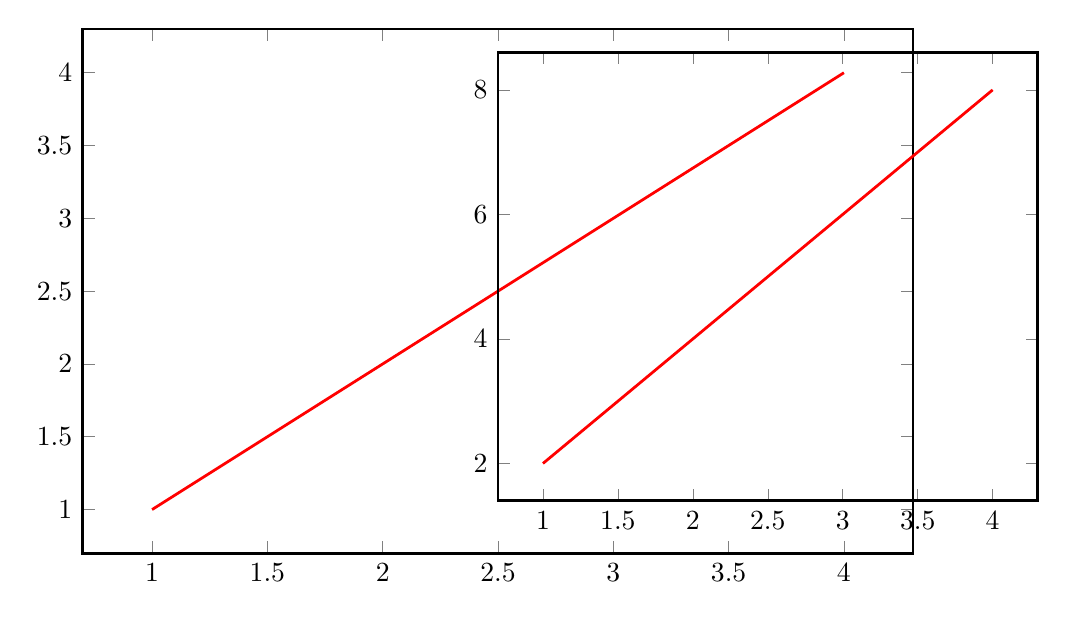
\begin{tikzpicture}
\usetikzlibrary{}
	\newlength{\mywidth}
	\setlength{\mywidth}{\columnwidth}
\begin{axis}[width=\mywidth,
	y post scale=0.75,
legend style={at={(0.95,0.95)},anchor=north east},
legend columns=1,
line width=1pt
]
\addplot[sharp plot,
solid,
red
] coordinates {
(  1.0000E+00,  1.0000E+00)
(  2.0000E+00,  2.0000E+00)
(  3.0000E+00,  3.0000E+00)
(  4.0000E+00,  4.0000E+00)
};
\coordinate (insetref0) at (rel axis cs: 0.5,0.1);
\end{axis}
\usetikzlibrary{}
\begin{axis}[at={(insetref0)},
width=\axisdefaultwidth,
height=\axisdefaultheight,
legend style={at={(0.95,0.95)},anchor=north east},
legend columns=1,
line width=1pt
]
\addplot[sharp plot,
solid,
red
] coordinates {
(  1.0000E+00,  2.0000E+00)
(  2.0000E+00,  4.0000E+00)
(  3.0000E+00,  6.0000E+00)
(  4.0000E+00,  8.0000E+00)
};
\end{axis}
\end{tikzpicture}

\end{document}
